\documentclass[11pt]{article}

\usepackage{amsmath}
\usepackage{amssymb}

\usepackage{graphicx}

\usepackage{ytableau}

\title{Catalan numbers, \\ Math 4707, Spring 2021}
\author{}
\date{}

\begin{document}

\maketitle

\vspace{-0.75cm}

The \emph{Catalan number} sequence 
\[C_0=1,C_1=1, C_2=2, C_3=5, C_4=14, C_5=42, \ldots,\] 
with general formula $C_n = \frac{1}{n+1}\binom{2n}{n}$, and generating function $C(x) := \sum_{n=0} C_n x^n$ given by $C(x) = \frac{1-\sqrt{1-4x}}{2x}$, is ubiquitous in combinatorics.

The Catalan numbers satisfy the \emph{fundamental recurrence} 
\[C_{n+1} = \sum_{k=0}^{n}C_k C_{n-k}.\]
 For each of the following possible definitions of $C_n$, explain why the fundamental recurrence holds:

\begin{enumerate}
\item $C_n := $ number of triangulations of an $n+2$-gon; the case $C_3=5$ corresponds to
\[
\includegraphics[width=10cm]{Catalan_number_triangulation.png}\]
\item $C_n := $ number of \emph{binary trees} (each node either has either two children: a left and a right child; or has no children and is a ``leaf') with $n+1$ leaves; the case $C_3=5$ corresponds to:
\[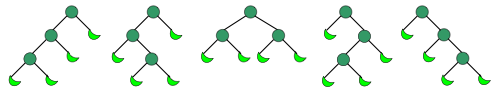
\includegraphics[width=10cm]{binary_tree.png}\]

\vspace{-0.2cm}
\item $C_n := $ number of words of length $2n$ with $n$ X's and $n$ Y's such that every initial segment has at least as many $X$'s as $Y$'s (these are called \emph{Dyck words}); the case $C_3=5$ corresponds to
\[\textrm{XXXYYY}  \qquad   \textrm{XYXXYY}  \qquad   \textrm{XYXYXY}  \qquad   \textrm{XXYYXY}  \qquad \textrm{XXYXYY}\]
\end{enumerate}

\pagebreak

For each of the following possible definitions of $C_n$, explain a bijection to one of the above definitions:

\begin{enumerate}
\setcounter{enumi}{3}
\item $C_n := $ number of lattice paths from $(0,0)$ to $(n,n)$ with steps $(0,1)$ and $(1,0)$ staying on or above diagonal $y=x$ (these are called \emph{Dyck paths}); case $C_3=5$:
\[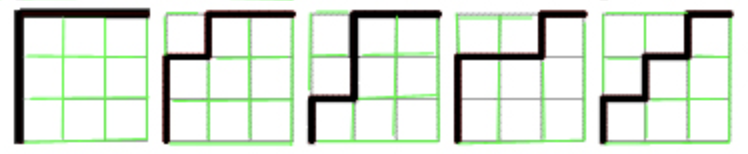
\includegraphics[width=10cm]{dyck_paths.png}\]
\item $C_n := $ number of ways to fill a $2\times n $ rectangle with the numbers $1,2,...,2n$ increasing in rows and columns; case $C_3=5$:
\[\begin{ytableau}1 & 2 & 3 \\ 4 & 5 & 6\end{ytableau}\qquad \begin{ytableau}1 & 2 & 4 \\ 3 & 5 & 6\end{ytableau} \qquad \begin{ytableau}1 & 2 & 5 \\ 3 & 4 & 6\end{ytableau} \qquad \begin{ytableau}1 & 3 & 4 \\ 2 & 5 & 6\end{ytableau} \qquad \begin{ytableau}1 & 3 & 5 \\ 2 & 4 & 6\end{ytableau}\]
\item $C_n := $ number of ways to completely parenthesize $n+1$ different factors; case $C_3=5$:
\[ \textrm{(((ab)c)d) } \qquad \textrm{((a(bc))d)} \qquad \textrm{((ab)(cd))} \qquad \textrm{(a((bc)d))}  \qquad \textrm{(a(b(cd)))} \]
\item $C_n := $ number of ways for $2n$ people seated at a circular table to shake hands without crossing; case $C_3=5$:
\[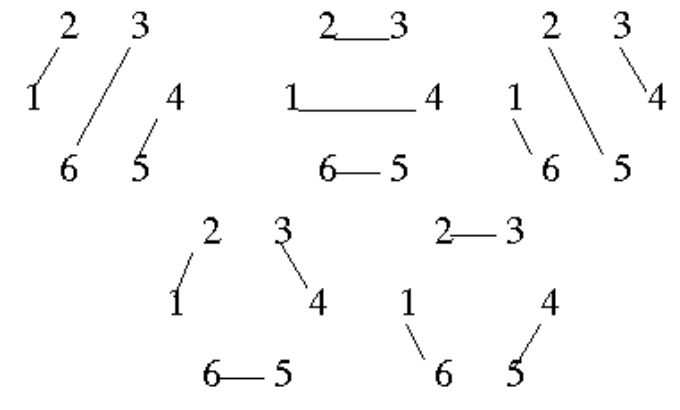
\includegraphics[width=7cm]{handshakes.png}\]

\end{enumerate}

\end{document}
